\documentclass[12pt]{article}
\usepackage[margin=1in]{geometry}
\usepackage{amsmath,amsthm,amssymb}
\usepackage{graphicx}
\usepackage{enumerate}
\usepackage{multicol}
\usepackage{caption}
\usepackage{subcaption}
\usepackage{booktabs}
\usepackage{hyperref}
\newcommand{\N}{\mathbb{N}}
\newcommand{\Z}{\mathbb{Z}}
\newcommand{\E}[1]{E\left[ #1 \right]}
\newcommand{\mbf}[1]{\mathbf{#1}}
\newenvironment{theorem}[2][Theorem]{\begin{trivlist}
\item[\hskip \labelsep {\bfseries #1}\hskip \labelsep {\bfseries #2.}]}{\end{trivlist}}
\newenvironment{lemma}[2][Lemma]{\begin{trivlist}
\item[\hskip \labelsep {\bfseries #1}\hskip \labelsep {\bfseries #2.}]}{\end{trivlist}}
\newenvironment{exercise}[2][Exercise]{\begin{trivlist}
\item[\hskip \labelsep {\bfseries #1}\hskip \labelsep {\bfseries #2.}]}{\end{trivlist}}
\newenvironment{problem}[2][Problem]{\begin{trivlist}
\item[\hskip \labelsep {\bfseries #1}\hskip \labelsep {\bfseries #2.}]}{\end{trivlist}}
\newenvironment{question}[2][Question]{\begin{trivlist}
\item[\hskip \labelsep {\bfseries #1}\hskip \labelsep {\bfseries #2.}]}{\end{trivlist}}
\newenvironment{corollary}[2][Corollary]{\begin{trivlist}
\item[\hskip \labelsep {\bfseries #1}\hskip \labelsep {\bfseries #2.}]}{\end{trivlist}}
\begin{document}
% --------------------------------------------------------------
% Start here
% --------------------------------------------------------------
\title{Project Report \\ \vspace{5mm} \large{COS 424: Interacting with Data}}
\author{Jonathan Balkind -- Santiago Cu\'ellar -- Jos\'e Ferreira -- Alex Tarr} 
\maketitle

%\begin{multicols}{2}

% Section 1. Introduction
\section{Introduction} 
Many companies working in e-commerce (Amazon), internet streaming (Netflix, Hulu), and business review sites (Yelp, Groupon) seek 
to make personalized recommendations to their users in order to enhance the user's experience. This is accomplished by recommendation systems, 
which use the knowledge of its users and items to make guesses on what items the user would enjoy. This problem is formulated as a matrix completion 
problem, where we are given a sparse matrix of ratings that users have given to items and seek to estimate the missing entries.
	One popular method used for recommendation systems is the latent factor model, which is a popular collaborative filtering method that found great 
	success in the well-known Netflix problem. This method seeks to characterize items and users on a set of unknown factors inferred from the rating patterns. 
	Applied to the matrix completion problem, the latent factor model attempts to factorize the ratings matrix into a set 
	of user vectors and item vectors, where the elements of the item vector can be interpreted as how much a specific factor characterizes the item, while elements 
	of the user vector represents how much the user likes items high on the corresponding factor. 


% Section 2. Models
\section{Models}

Matrix factorization (MF) methods have been extensively used in recommender systems \cite{koren09}. The idea is that we can characterize users and businesses by a feature vector in the same (relatively) low-dimensional latent space. Ideally, the features would represent meaningful dimensions that determine the characteristics of a business or user. However, matrix factorization techniques usually result in uninterpretable features. 

Nevertheless, in some sense, they perform operations akin to a singular value decomposition (SVDs) with the added advantages that it does not require a dense matrix , and that it is substantially less computationally expensive. SVD would require one to guess the missing values (imputation), as well as adding great computational expense to the problem. We next present the models used to assess the applicability of matrix factorization to the problem at hand (more details can be found in the Technical Appendix).

\paragraph{Model 1.} In sum, we want to factorize the very large sparse ratings matrix of users \emph{vs.} businesses into two oblong matrices $\mbf U\in\mathbb{R}^{n_u\times f}$ and $\mbf B\in\mathbb{R}^{n_b\times f}$, where $f$ is the number of latent factors. The important point is that we only wish to consider the ratings that we do have (thus ignoring all the unknown ratings). Therefore, we wish to find $\mbf U$ and $\mbf B$ that solve the following optimization problem:
\begin{equation}
\min_{\mbf U,\mbf B} = \sum_{(i,j)\in K} (r_{ij}-\mbf u_i^T\mbf b_j)^2+\lambda\left(||\mbf u_i||^2+||\mbf b_j||^2\right)
\end{equation}
where $K$ is the set of non-empty ratings in the matrix and the $\mbf u_i$ and $\mbf b_i$ are feature vectors associated with user $i$ and business $j$, respectively (columns in $\mbf U$ and $\mbf B$). The regularization parameter helps prevent overfitting (in a sense, accounting for the prior belief that most ratings are somewhat fair). With this model, we can easily predict a new rating using:
\begin{equation}
\hat r_{ij} = \mbf u_i^T\mbf b_j.
\end{equation}

\paragraph{Model 2.} Unfortunately, model 1 is rather restrictive. In particular, it doesn't account for user and business biases which one would expect to play a big role in defining the true ratings. As such, we consider a new prediction model:
\begin{equation}
\hat r_{ij} = \mu + p_i + q_j + \mbf u_i^T\mbf b_j
\end{equation}
where $\mbf p$ and $\mbf q$ represent average user and business biases, respectively, and $\mu$ is the global average rating. The optimization problem to be solved changes accordingly, and is now over $\mbf U$, $\mbf B$, $\mbf p$ and $\mbf q$ (see Technical Appendix for details).

\paragraph{Model 3.} Another model one can consider stems from the realization that business average ratings tend to represent a better baseline than user ratings in the Yelp dataset (as there is a large number of users that have a small amount of ratings). As such, it is helpful to consider a prediction model of the following form \cite{funk06}:
\begin{equation}
\hat r_{ij} =  p_i + q_j + \mbf u_i^T\mbf b_j
\end{equation}
where $q_j$ now represents the average rating for business $j$ and $p_i$ is the average rating offset for user $i$. Note that in this model we are only optimizing over the matrices $\mbf U$ and $\mbf B$. 

\paragraph{Model BL.} In order to directly assess the effectiveness of the matrix factorization technique, we compared the results against a baseline model using Model 3's framework without the factorized matrices. This requires no optimization.

\paragraph{Linear Models (including Lasso and Ridge)} We include three Linear Models to test their performance in comparison to the MF techniques. The prediction equation is simply $\hat r_{ij}=\mbf x_{ij}^T\boldsymbol\theta$ with parameter vector including: average rating from user $i$, average rating received by business $j$ and a collection of meta-data about business $j$. The model is fitted using MLE. The Lasso model is regularized using the $\ell_1$-norm, which seeks a sparse solution that picks out the most meaningful features that constitute the regressor set. The Ridge model is regularized using the $\ell_2$-norm, which seeks to reduce the size of the coefficients and prevent overfitting.

% subsection on error analysis
\subsection{Results and Error Analysis}
The parameters $\lambda$ and the number of latent factors were chosen through 10-fold cross-validation. Two metrics were considering for assessing the quality of the model: root mean squared error (RMSE) and mean absolute error (MAE). We also computed precision for the best out of our three MF models, as well as for the BL model.

The results obtained for each of the models can be seen in Table \ref{tab:results} below. We note that the factorized models fared worse than the simple baseline model. Below, we address some of the reasons that may explain these results.

\paragraph{Sparsity.} While the popularity of MF methods came about in the context of sparse ratings matrices, we suspect that excessive sparsity has substantial negative impact on the performance of the model. In particular, 83\% of the users in the training set have less than 5 reviews to their name and 49\% have a single review. The text associated with these reviews is, more often than not, descriptive of either an excellent experience or a terrible one. It appears that many of the users have created accounts solely for the purpose of writing a single extreme review, the effect of which is not accurately portrayed by our models.

\paragraph{Critic users.} We took the vector $\mbf p$ of average user offsets from Model 3 and used it to split the users into three groups: positive, negative and fair (see Figure \ref{fig:user_offsets}). We then used the partitioned ratings matrix to fit three factorization models using Model 3. The cluster information and results obtained can be found in Table \ref{tab:results_clusters}. We note that the average error did not change much for fair users. However, positive users saw a substantial improvement in MAE. This is likely a result of the positive bias in the ratings, as seen in Figure \ref{fig:hist_ratings} and the fact that our prediction model clips the ratings to the interval $[0,5]$. More worrying, however, was the decrease in performance for negative users. Unlike with the positive users, this does not appear to result from clipping, but rather from intrinsic variance in the ratings from these users. This suggests that it would be useful to employ different levels of regularization depending on the average offset of the user (future work).

\paragraph{Businesses.} Interestingly, the number of ratings businesses have does not appear to correlate positively with prediction accuracy (in the extremes of performance). We considered businesses with high accuracy predictions (RMSE$\leq$0.5) and those with low (RMSE$\geq$1.5). The set of low accuracy businesses had, on average, about 18 reviews, while the high accuracy set had about 13. However, we did see the same pattern as in users in the sense that the high accuracy set had a high average rating ($\approx4.1$) while the low average set had a lower rating ($\approx3.2$).

\subsection{Imputation}  
Given Model 3 proved to be the most successful of the three MF models considered, we attempted to better account for priors by filling in random ratings for users with 5 or less reviews (until they totalled 5 reviews). The filled-in values were just the business averages. Fitting Model 3 to this new ratings matrix resulted in modest improvements (see Table \ref{tab:results}), and it is possible that picking the number of reviews to fill in more carefully could yield greater improvements. 

\subsection{Linear Models}
The linear models we introduced each achieve comparable performance to the factorized models. In particular, the linear model and ridge nodel both perform as well as the imputation model, though still not as well as the Model BL either in terms of RMSE or MAE.

\section{Clustering the businesses}
We noticed, by reading some reviews, that people rate different kinds of business in radically different ways. %Maybe add examples? 
We believe that due to such differences in the nature of businesses, a user's review of a hair salon might not correlate with their preference of pizza place\footnote{Admittedly there might be an interesting correlation! But we think it's not a linear relation that would help this project.}.
With that in mind, we want to group similar businesses together and then try to produce separate predictions on each group. To do so, we use the businesses' attributes, or meta-data, to cluster them.

The business meta-data is a list of attributes that describe some of its characteristics. Most of the entries are boolean values such as \emph{Wheelchair Accessible} or \emph{Accepts Credit Cards}. Some other entries are natural numbers, such as \emph{review count} and \emph{Price Range}, or more general such as \emph{Hours}--wich describes hours of service. Moreover, businesses can have a section with categories such as \emph{Women's Clothing} or \emph{Mexican food}.

The main challenge here is that most businesses have their metadata incomplete. Moreover, most of the attributes are only applicable to restaurants, such as \emph{Good for lunch} or \emph{takes reservations}\footnote{some hair salons take reservations, but you get the point.}. On the other hand, most businesses have categories, but each business is in many of the more than 500 categories. So categories alone were not enough for classification. 

Our solution was to encode all the meta-data available in a feature vector for each business and use a clustering algorithm with that information. The feature vectors have more than 600 entries and we computed 30 clusters. We use the standard Lloyd's algorithm \cite{lamport94} to perform k-means clustering on the businesses.  

A sample of the results can be observed in table \ref{clusters2}. Just like the sample presented, each cluster featured, in general, very similar businesses with some clear features in common. Our algorithm distinguished very particular categories into a single cluster, (such as \emph{hospitals}) but also managed to merge similar categories such as \emph{chicken wings} and \emph{sandwiches}.


\subsection{Factorizing the clusters}

Once we separated our businesses into groups of similar attributes, we tried to solve the original problem on each individual cluster. To do so, we create new sparse matrices for each group and factorize them with method 2 described above. 

The first clear improvement was on the runtime and the memory requirements. Since the matrices are much smaller, they take less space in memory (around $\frac{1}{30}$ of the memory) and they can be factored in parallel, making the factorization process about 5 times faster. We think this is crucial to make this algorithm scalable, but we will not go into a detailed analysis of the runtimes in this project.

Some of the numeric results are summarized in table \ref{clustersFact}. Some clusters showed a significant improvement ( up to \emph{rmse} $= 1.1560$) and others performed much worse ( \emph{rmse} $= 1.7801$). The overall performance was not better than that of factorization on the entire matrix (\emph{rmse} $= 1.4638 $).

We did not find any relationship between the performance of the factorization and the size of the matrix, the category of the cluster or the number of samples on the test set. 

\section{Conclusion}

In this project we explored the problem of matrix completion using a very sparse dataset of businesses and user reviews. We made extensive use of matrix factorization, with overall poor results. Incorporating the meta-data about the businesses through clustering did not improve the performance of the MF techniques. In most cases, the results worsened.

We believe one of the main reasons for this poor performance arises from the large number of users with very few reviews. There is also a large positive bias in reviews, which improves the results for highly rated businesses, but damages the overall fit of the model. 

The MF models appear to require extensive fine-tuning of parameters, which is not the case with simpler models (such as a linear regression model). It is unclear whether more careful parameter tuning would make the MF methods competitive. However, the linear models requires little tuning and produced comparable results with considerably lower computational requirements, making them a more attractive option for solving the recommendation problem.

%\section{Bibliography}
\begin{thebibliography}{9}

\bibitem{lamport94}
  Lloyd, S.,
  \emph{Least squares quantization in PCM}.
  Information Theory, IEEE Transactions on
  p. 129-137
  1982.

\bibitem{koren09}
  Koren, Y., Bell, R., and Volinsky, C
  \emph{Matrix Factorization Techniques for Recommender Systems}
  Computer
  p. 30-37
  2009.

\bibitem{funk06}
  Funk, S.
  \emph{Netflix Update: Try This at Home}
  \url{http://sifter.org/~simon/journal/20061211.html}
  Dec, 2006.

\end{thebibliography}
%\end{multicols}



% Results Appendix
\newpage

% Table generated by Excel2LaTeX from sheet 'Sheet1'
\begin{table}[htbp]
  \centering
  \caption{Best root mean squared error and mean absolute error results for each model (parameters chosen through 10-fold cross-validation).}
    \begin{tabular}{rrrccc}
    \toprule
          & Parameters & RMSE  & MAE & Precision \\
    \midrule
    Model 1 & $\lambda=0.05$,$f=20$ & 1.3359 & 1.0210 & -- \\
    Model 2 & $\lambda=0.30$,$f=20$ & 1.2033 & 0.9113 & --\\
    Model 3 & $\lambda=0.20$,$f=20$ & 1.1913 & 0.9163 & 0.8266\\
    Model 3 + Imputation & $\lambda=0.20$,$f=10$ & 1.1772 & 0.903  & --\\
    Linear Model & $\theta$ & 1.1754 & 0.9073 & --\\
    Linear Model (Lasso) & $\theta$ & 1.2523 & 1.0104 & -- \\
    Linear Model (Ridge) & $\theta$ & 1.1753 & 0.9074 & --\\
    Model BL & None & 1.1517 & 0.8972 & 0.8444 \\
    \bottomrule
    \end{tabular}%
  \label{tab:results}%
\end{table}%

% Table generated by Excel2LaTeX from sheet 'Sheet1'
\begin{table}[htbp]
  \centering
  \caption{Best root mean squared error and mean absolute error using Model 3 for three user clusters: positive ($\text{mean}(p_i)=0.44$), neutral ($\text{mean}(p_i)=0.03$), negative ($\text{mean}(p_i)=-0.67$).}
    \begin{tabular}{rrr}
    \toprule
          & RMSE  & MAE \\
    \midrule
    Negative Users & 1.4567 & 1.1835 \\
    Neutral Users & 1.1808 & 0.9098 \\
    Positive Users & 1.1643 & 0.7957 \\
    \bottomrule
    \end{tabular}%
  \label{tab:results_clusters}%
\end{table}%

\begin{figure}
	\centering
	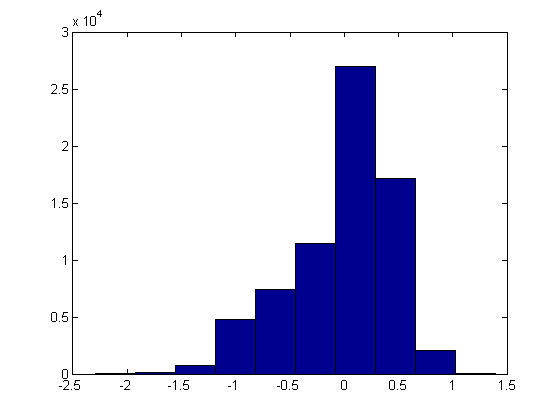
\includegraphics[scale=0.5]{user_offsets.png}
	\caption{Histogram of average user offsets in the training set.}
	\label{fig:user_offsets}
\end{figure}

\begin{figure}
	\centering
	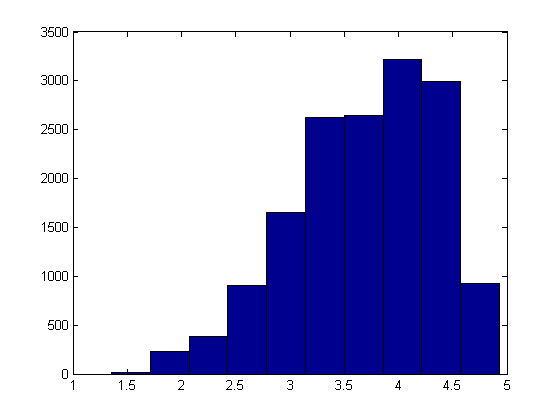
\includegraphics[scale=0.5]{hist_ratings.png}
	\caption{Histogram of ratings in the dataset.}
	\label{fig:hist_ratings}
\end{figure}


\newpage 
% Table generated by Excel2LaTeX from sheet 'Sheet2'
\begin{table}[htbp]
  \centering\scalebox{1}{
    \begin{tabular}{rcc}
    \toprule
          & RMSE  & MAE \\
    \midrule
    Cluster Best RMSE & 1.1560 & 0.9116 \\
    Cluster Best MAE & 1.1981 & 0.7835 \\
    Cluster Worst RMSE and MAE & 1.7801 & 1.4263 \\
    Overall Error & 1.4638 & 1.1069 \\
    \bottomrule
    \end{tabular}%
  }\caption {Best, worst and overall performance of cluster factorization.}\label{clustersFact}
\end{table}%

% Table generated by Excel2LaTeX from sheet 'Sheet1'
\begin{table}[htbp]
  \centering\scalebox{0.6}{
    \begin{tabular}{rrrrr}
    \toprule
    \multicolumn{5}{c}{\Huge Some examples of clusters} \\
    \midrule
    PetSmart & Blue Sky Java & Bertha's Café & Armadillo Grill & Hermosa Inn \\
    Katz \& Dogs Wellness Clinic & It's A Grind Coffee House &  Sweet Cakes Café & Belvedere American Bar \& Grill & Super 8 Phoenix \\
     Vetcare Internal Medicine &  Starbucks Coffee &  Schlotzsky's & Arcadia Tavern & Phoenix Airport Marriott \\
     Poochie's Pet Grooming &  Starbucks Coffee & Jimmy John's & The Tavern On Mill & Residence Inn by Marriott \\
     Doggie Door &  Starbucks Coffee & Market Bistro & Hooters & Phoenix Marriott Mesa \\
     PetSmart &  Starbucks & Bagel Nosh & Famous Sam's & Hampton Inn Surprise \\
     Small Animal Clinic &  Starbucks & Jimmy John's & Half Moon Sports Grill & Motel 6 \\
     VCA Phoenix West Animal Hospital & Rich Aroma Coffee Co & Sandwich Club & Barfly & Super 8 Mesa / Gilbert \\
     Pride Animal Hospital & Starbucks & Subway & Gallagher's & Motel 6 \\
     Dog Days & Dutch Bros Coffee & Einstein Bros Bagels & Islands Restaurant & Hilton Suites-Phoenix Plaza \\
     Brambley Hedge Rabbit Rescue & Seattle Espresso & Nielsen's Frozen Custard & SJ's Sports Grill & Ramada Tempe \\
     Phoenix Mountain Animal Hospital &  TeaGschwendner & Port of Subs & Buffalo Wild Wings & Ramada Peoria \\
     Play All Day! Pet Care & Starbucks Coffee & The Original Hoagie Shop & The Lodge & Scottsdale Resort Club \\
    Tranquility Trail Animal Sanctuary & Starbucks & Grinders Coffee Company & Native New Yorker & Comfort Suites Phoenix \\
     Bargain Barks & Starbucks & Vovomeena & Jt's Bar \& Grill & Motel 6 \\
     R.E.S.C.U.E. & Starbucks Coffee Company &  Niki's Kitchen- Fry Bread & Native New Yorker & Homewood Suites \\
     Cochise Animal Hospital & Starbucks & Wildflower Bread Company & Library Bar \& Grill & Sleep Inn Mesa \\
     Top Dog Grooming & Starbucks Coffee &  Port of Subs & Chili's Grill \& Bar & Clarion Hotel \\
     TLC House \& Pet Sitting Service &  Starbucks Coffee & Cave Creek Coffee Company & Mad G's Grill \& Tavern & Extended Stay America \\
     Choice Pet Market &  Arizona Coffee Connection & Mr. Goodcents Subs \& Pastas & Horse \& Hound Sports Grill & Best West Inn \\
     Gordon's Feed \& Seed & Starbucks & Short Leash Dogs Food Truck & The Monastery Mesa & Fairfield Inn by Marriott \\
     See Spot Shop & Starbucks Coffee & Blimpie Subs \& Salads & Boulders On Broadway & Hyatt Place \\
     Paws Salon & Starbucks & Rumbi Island Grill & ZuZu at Hotel Valley Ho & Windmill Inns \& Suites \\
     Dolittle Dog Grooming &  The Street & Express Donuts & Teakwoods Tavern and Grill & Holiday Inn \\
     Tempe Veterinary Hospital &  Bosa Donuts & Fujiya Market & Starters Sports Bar and Grill & Springhill Suites by Marriott \\
     Ray's Feed Store &  Teavana &  Essence Bakery Café & Rimrock Bar \& Grille & Crossland Economy Studios \\
     Banfield Pet Hospital &  Starbucks Drive Thru & Philly's Famous & The Vig & Homewood Suites Phoenix \\
     Preppy Pet Phoenix North & WhereUBean Coffee &  Franks A Lot & Dave \& Buster's & Radisson Hotel \\
     PetSmart & It's A Grind Coffee House &  Jersey Mike's & Copper Still Moonshine Grill & Comfort Suites \\
    \bottomrule
    \end{tabular}%
}\caption {Some examples of clusters}\label{clusters2}\end{table}%



% Technical Appendix
\newpage
\section{Technical Appendix}
This section provides a few additional details on the matrix factorization technique. 

The solution of each of the optimization problems follows from simple gradient descent (learning rate parameter $\gamma$). We consider each model in turn and present the optimization problem to be solved as well as the update equation that results.

\paragraph{Model 1} The optimization problem for this model is:
\begin{equation*}
\min_{\mbf U,\mbf B} = \sum_{(i,j)\in K} (r_{ij}-\mbf u_i^T\mbf b_j)^2+\lambda\left(||\mbf u_i||^2+||\mbf b_j||^2\right)
\end{equation*}
and results in the following simple update equations
\begin{equation*}
\mbf u_i \leftarrow \mbf u_i+\gamma\left(e_{ij}\mbf b_j-\lambda\mbf u_i\right)
\end{equation*}
\begin{equation*}
\mbf b_j \leftarrow \mbf b_j+\gamma\left(e_{ij}\mbf u_i-\lambda\mbf b_j\right).
\end{equation*}
where $e_{ij}\equiv r_{ij}-\hat r_{ij}$.

\paragraph{Model 2} The optimization problem is:
\begin{multline*}
\min_{\mbf U,\mbf B,\mbf p,\mbf q} = \sum_{(i,j)\in K} (r_{ij}-\mbf u_i^T\mbf b_j-p_i-q_j-\mu)^2\\
+\lambda\left(||\mbf u_i||^2+||\mbf b_j||^2+p_i+q_j\right)
\end{multline*}
so that we have two additional update equations:
\begin{equation*}
p_i\leftarrow p_i+\gamma\left(e_{ij}-\lambda p_i\right)
\end{equation*}
\begin{equation*}
q_j\leftarrow q_j+\gamma\left(e_{ij}-\lambda q_j\right).
\end{equation*}

\paragraph{Model 3} The optimization problem is:
\begin{multline*}
\min_{\mbf U,\mbf B} = \sum_{(i,j)\in K} (r_{ij}-\mbf u_i^T\mbf b_j-p_i-q_j)^2+\\
\lambda\left(||\mbf u_i||^2+||\mbf b_j||^2\right).
\end{multline*}
The update equations are similar to the ones for Model 1. We note that to estimate $\mbf p$ and $\mbf q$ from the data, we should account for priors. This prevents attributing excessive importance to individual ratings when the users (or businesses) have a small number of ratings. Therefore, for business $j$, we obtain:
\begin{equation*}
q_j = \frac{R \mu+\sum_i r_{ij}}{R+\sum_i\mbf 1\{r_{ij}\neq 0\}}
\end{equation*}
where $R$ is the ratio between the overall variance and the variance of the business mean ratings. The same technique is employed for estimating $\mbf q$.


\end{document}




 